\subsection{Self-confidence Factorization} \label{sec:self-confidence}

\famsec{} represents and computes self-confidence through functions that score different parts of an autonomous agent's decision-making process, referred to as \emph{self-confidence factors}. The combined set of self-confidence factors provide a meta-analysis of how operations and approximations inherent to the agent's decision-making process are expected to impact it's overall task performance. 
As with the self-confidence reporting strategy developed in \cite{Hutchins2015-if}, the factors ideally encode an expert designer's assessment of the reliability and suitability of an autonomous decision-making system for completing a task, accounting for variations and uncertainties in task specification, context, environment, and system implementation. \famsec{}'s novelty is that it allows autonomous decision-makers to automatically generate self-confidence assessments from information that is already available from setting up and solving the task at hand. Thus, unlike \cite{Hutchins2015-if}, human experts are not needed to assign specific self-confidence values a priori for every possible tasking scenario that the decision-maker could encounter. %% (contrast to other self-confidence methods later on -- none which specifically look at decision-making, and \famsec allows different concepts to fall into one umbrella framework...) 
    
    
\begin{figure}[tbp]
        \centering
        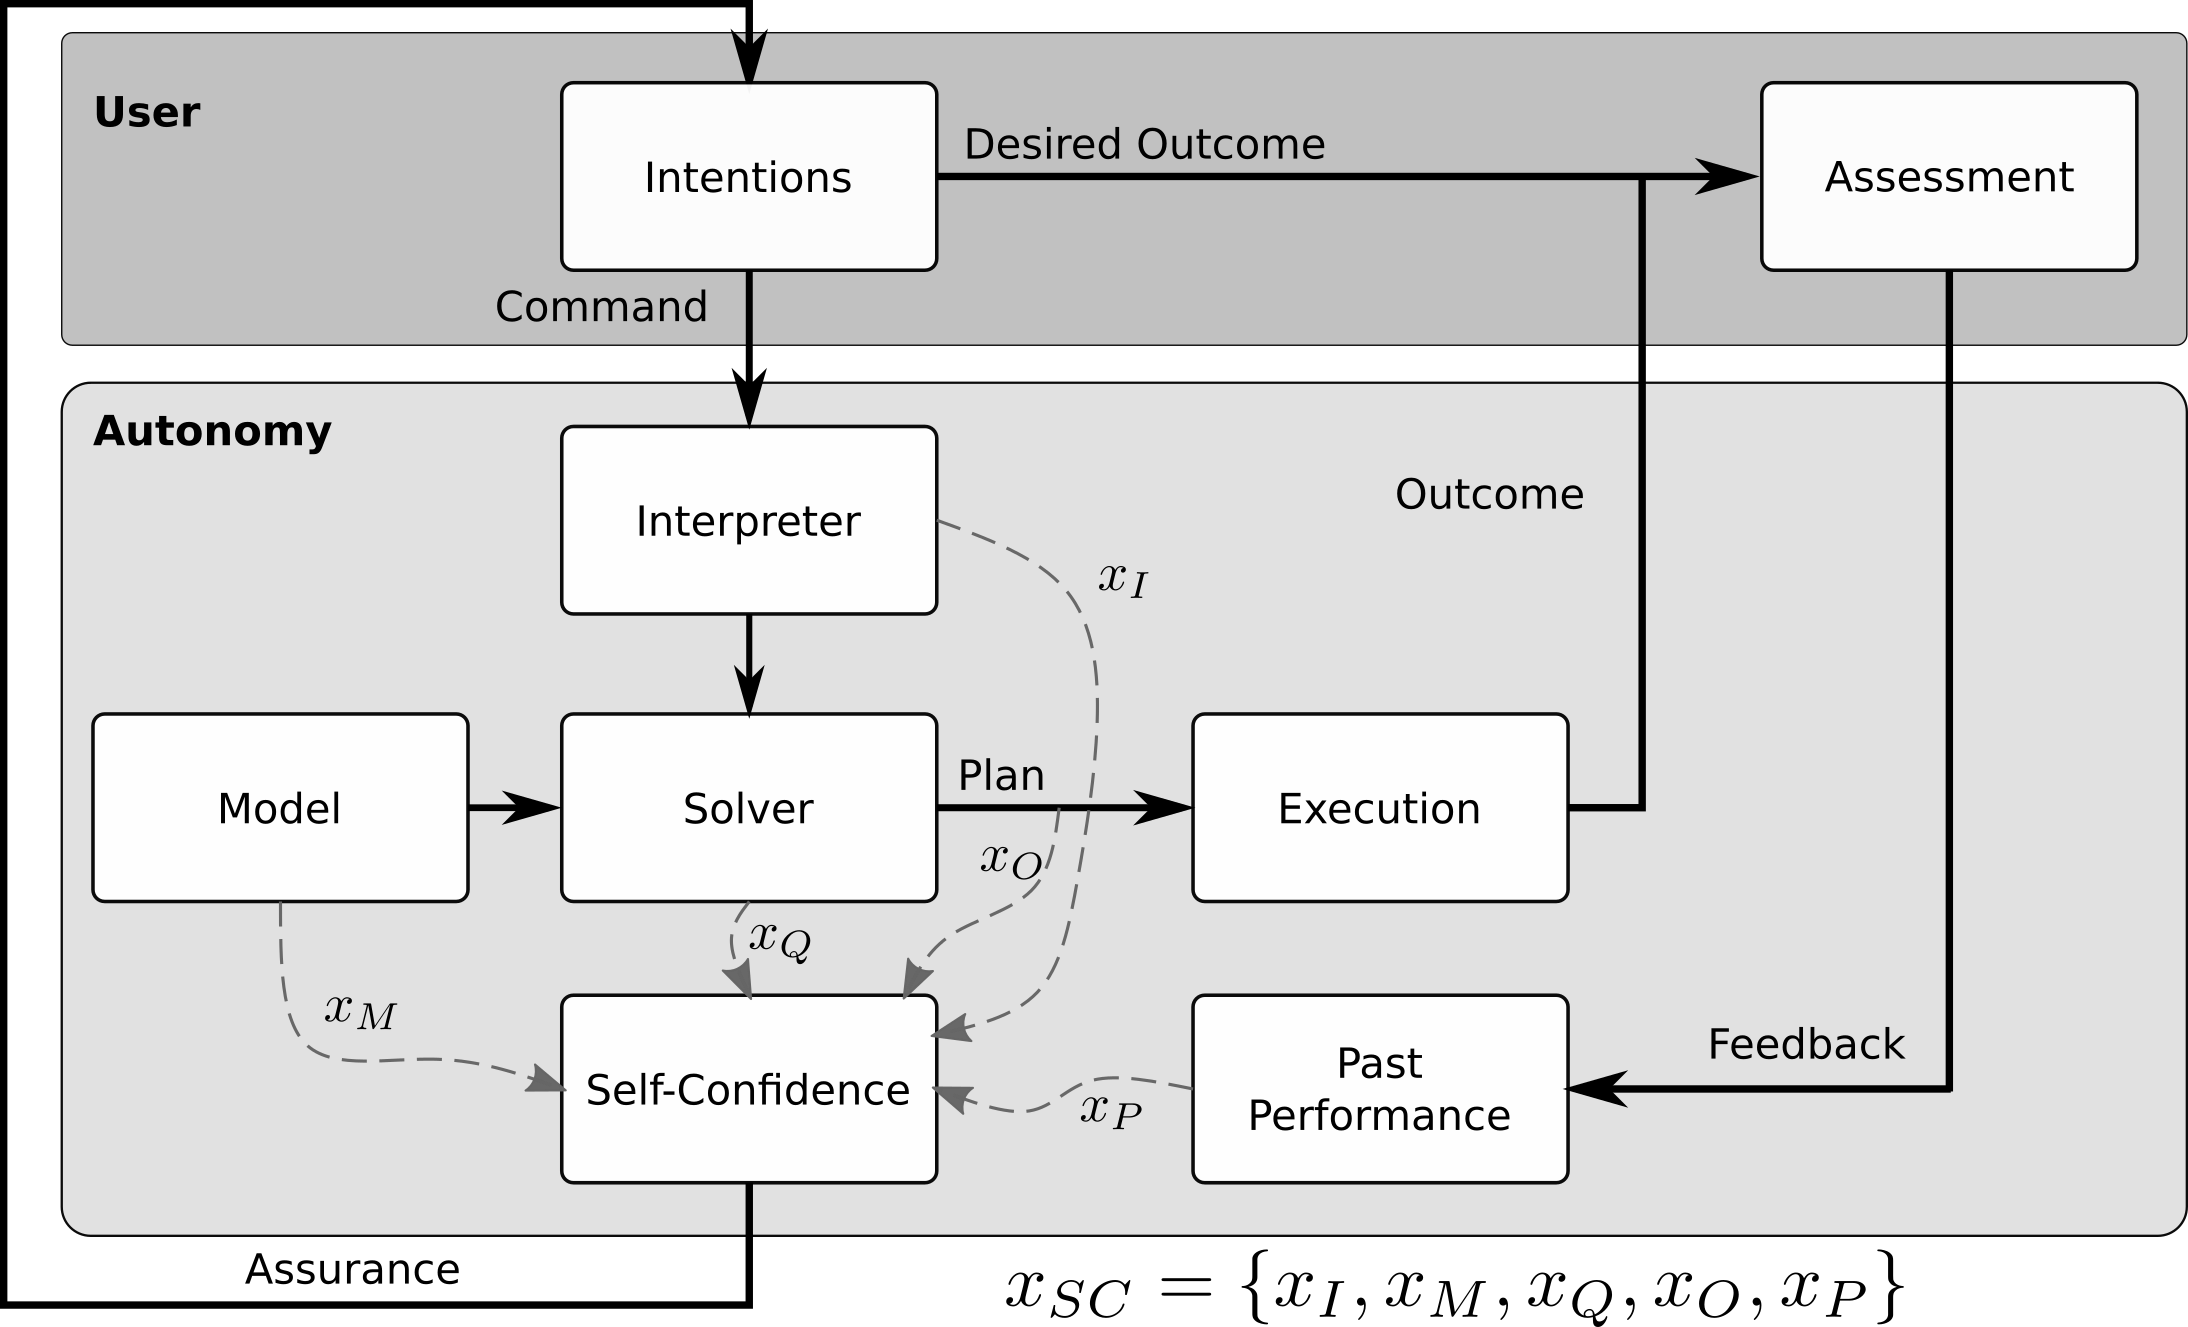
\includegraphics[width=0.85\linewidth]{Figures/FaMSeC.png}
        \caption{\famsec{} information flow}
        \label{fig:famsec}
        \vspace{-0.5 cm}
\end{figure}
    
Figure \ref{fig:famsec} illustrates a notional view of \famsec's overall self-confidence scoring mechanism. The self-confidence factors (dashed lines) are derived from core algorithmic decision-making components (white boxes in the `Autonomy' block).  
Each factor can be mapped onto an arbitrary scale, e.g. -1 to +1 for the sake of discussion, where -1 gives a shorthand indication of `complete lack of confidence' (i.e. some aspect of task, environment, or context falls completely outside the system's competency boundaries), and +1 indicates `complete confidence' (i.e. all aspects of task, environment, and mission context are well within system's competency boundaries). 
The scales for each factor need not all be the same and can carry slightly different qualitative interpretations, as long as a clear sense of `confidence direction' (i.e. degree of self-trust) can be established for each. Ref. \cite{Aitken2016-cv} considers five general self-confidence factors for autonomous decision-making: %that contribute to a `total self-confidence score', which notionally maps the combined set of factors into an overall confidence report:
\begin{itemize}
    \item \xI---\textit{\textbf{interpretation of user intent and task}}: to what extent were the user's intentions properly understood and translated by the autonomous robot into context-appropriate problem specifications and tasks?; 
    \item \xM---\textit{\textbf{model and data validity}}: are the robot's learned and/or assumed models, and training data used for decision-making `good enough' proxies for the real world?; 
    \item \xQ---\textit{\textbf{solver quality}}: are the approximations and learning-based adaptations used by the robot for solving decision-making problems appropriate for the given mission and model?; 
    \item \xO---\textit{\textbf{expected outcome assessment}}: do the sets of possible events, rewards, costs, utilities, etc. for a particular decision lead to a desirable landscape of possible task outcomes?; 
    \item \xP---\textit{\textbf{past history and experiences}}: what can be gleaned from the robot's own experience and other available information for past problem instances? %%\brett{refer to \cite{Israelsen2018-qz} for more detail if we feel we need it}
\end{itemize}

These factors could also be combined to produce a total self-confidence score that acts as a simple shorthand signal for users, which can then be parsed further as needed. 
Since the overall self-confidence mapping is heavily dependent on application, context, and desired levels/types of user-autonomy interaction, this work assumes for simplicity that the overall mapping consists of a direct report of all or some fixed subset of the component factors. %, e.g. \xSC. 
Furthermore, the five factors considered here are not necessarily exhaustive. For example, the factors as defined above are primarily aimed at meta-analysis of decision-making \emph{prior} to the execution of a particular task, whereas it is conceivable that other self-confidence factors could be included to account for in situ and post hoc analyses. Attention is restricted here to the a priori self-assessment case. With these concepts and caveats in mind, the remainder of this paper focuses on how \famsec{} can be applied in cases where the algorithmic decision-making components in Fig. \ref{fig:famsec} correspond to an MDP-based autonomous robot. 

\subsection{\famsec{} for MDP-based Autonomy} 
We will use the MDP framing of the Donut Delivery problem described earlier to illustrate the role of these factors and the relationships between them, as well as to examine three core questions: (i) how are the factors expected to behave under different conditions (independently of how they are calculated)?; (ii) how should these factors actually be calculated?; and (iii) ...\nisar{clean up:} what good is it for human users anyway? 

To address (i): if we suppose some class of MDP solver is available for the underlying ADT navigation problem, then we can examine expected trends, sensitivities, and interactions for the various self-confidence factors in relation to specific features of problem instances and MDP solver instances. 
For example, if the problem were modeled  as a discrete-time/discrete-space MDP, then value iteration could be used to find the optimal policy $\pi$, or sampling-based Monte Carlo solvers could be used to find an approximately optimal policy $\tilde{pi}$ \cite{Browne2012-lj}. In either case, the policy would map joint ADT-MG state information onto specific actions to maximize the ADT's expected cumulative discounted reward. \nisar{should this last sentence go in Sec. II??} 
Figure \ref{fig:trendsBCs} shows some expected behaviors for the \famsec{} factors as a function of task, environment, system, and context when a hypothetical Monte Carlo solver is used, assuming again an arbitrary finite range of -1 (total lack of confidence) to +1 (complete confidence). For instance, \xQ{} would be expected to increase/decrease as the number of samples used by the Monte Carlo solver to approximate $\pi$ increased/decreased. Similar trends can also be derived for other solver types (e.g. applying the result of value iteration prior to satisfactory convergence from an arbitrary initial condition would likely produce a poor estimate of the optimal policy). %\nisar{mention about traceability/drill down basis here?}
\begin{figure}[tbp]
    \centering
    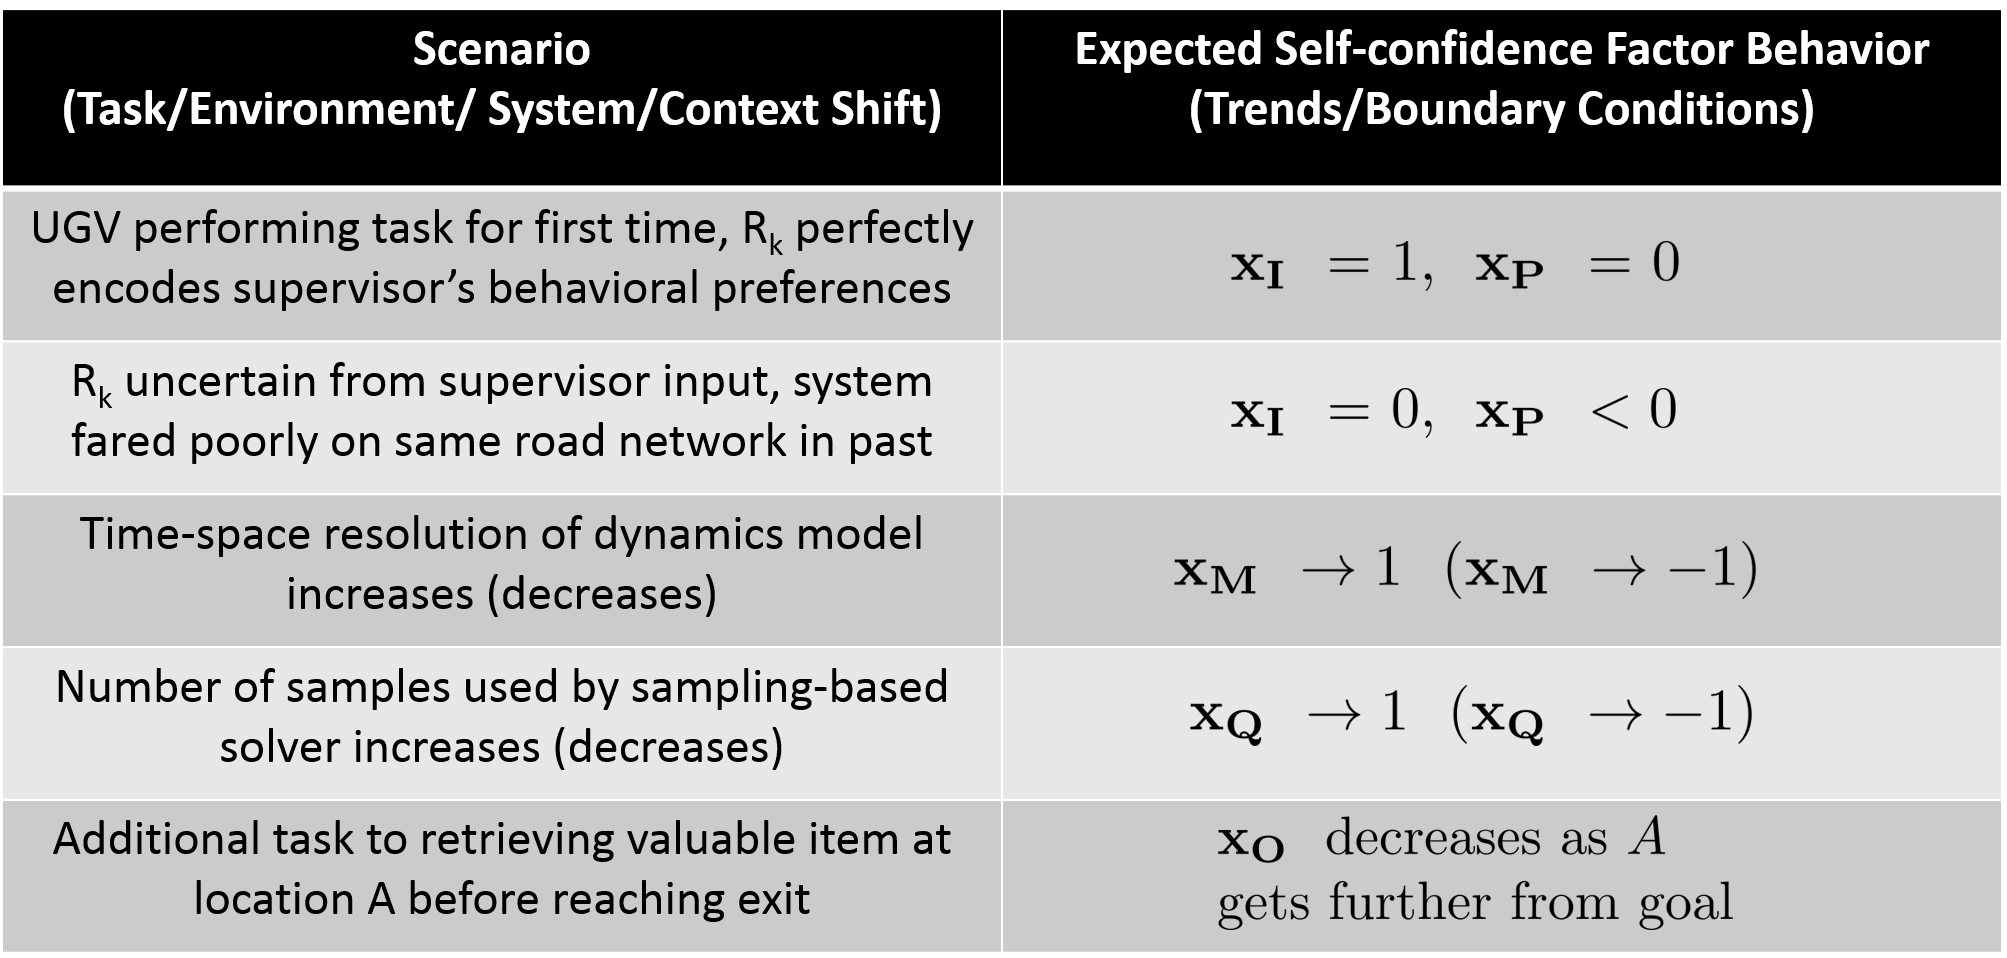
\includegraphics[width=0.65\linewidth]{Figures/scTrendsBoundaryExample_2generic.png}
    \caption{Notional \famsec{} factor behaviors for Donut Delivery problem. \nisar{try to combine this with \famsec{} block diagram somehow to save space?} }
    \label{fig:trendsBCs}
    \vspace{-0.5 cm}
\end{figure}

These expected behaviors for an MDP-based autonomous robot provide a useful starting point for developing formal definitions and computing strategies for specific self-confidence factors that address question (ii). 
An important issue to consider here of course is that the factors can co-vary with each other in complex ways. \nisar{say something about how logically stacked/asymmetric these are, i.e. bad solver implies lack of confidence in outcome, but not vice-versa...? }
As mentioned in \cite{Aitken2016-cv}, a logical simplifying assumption for initial algorithm development is to consider cases where we can ignore the interactions between factors. 
This is equivalent to examining each factor along `boundary conditions' where other factors do not change and thus have little/no contribution to the overall self-confidence score. 
We review next how ref. \cite{Aitken2016-cv} used this approach to develop a principled definition and calculation method for \xO{} in the context of MDPs. Then, to address the open problems of how other factors can be computed and how different factors interact when the boundary condition assumptions are relaxed, we present a new formal definition and strategy for computing \xQ{} with MDPs which naturally accounts for interactions with \xO{}.  %%that arise when the boundary condition assumptions are relaxed. 
\nisar{clean up...} ...Finally, to address question (iii) with these pieces of famsec in place, we present human experiment trials in Sec. blah... 

%Furthermore, studies with human users have not yet been done to validate and evaluate the impact of self-confidence reporting on task delegation. The remainder of the paper addresses both gaps. 
